%%\newpage
\begin{problem}{\textbf{\textsc{Coilfun}}}
Consider an air-cored superconducting solenoid of length $l = 1\;\mathrm{m}$ with cross-sectional area $A = 0.1 \;\mathrm{m}^2$ and $N = 1000$ turns. We connect the ends of the solenoid to each other with superconducting wires and run a current $I  = 1600\;\mathrm{A}$ through the entire setup. Assume that the solenoid behaves ideally. 
\newline
\newline
Cosmonaut Carla has a core with the same dimensions as the solenoid. The core has relative permeability $\frac{\mu_i}{\mu_0} = 10000$ and mass $10\;\mathrm{kg}$. The core is released at rest far from the solenoid and, due to magnetic forces, flies through the solenoid. Cosmonaut Carla can choose to quench the solenoid (instantaneously removing the current) at any time. What is the maximum attainable exit velocity of the core? 


\FloatBarrier
\begin{figure*}[!htbp]
\centering
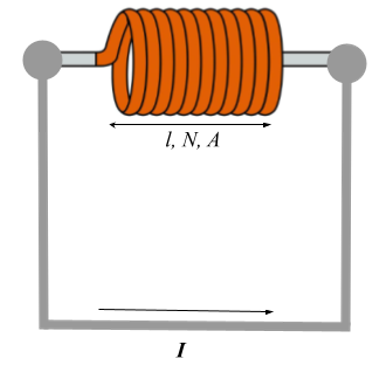
\includegraphics[width=0.3\textwidth]{problems/figures/coilfun.png}
\end{figure*}
\FloatBarrier

\end{problem}